\section{Standortenkodierung}
Als Standort wird ein einzigartiger diskreter Ort im Indoor-Szenario bezeichnet.
Bei der Klassifizierung können Standorte auf verschiedenen Arten im ML-Modell enkodiert werden.
Mian enkodierte die Pfade zwischen Interessepunkten als Standorte,
d. h. das Klassifizierungsergebnis ist der Pfad auf dem sich der Mikrocontroller befindet \cite{naveedThesis}.
\newline
\newline
Daneben wurden in dieser Arbeit noch zwei weitere Ansätze untersucht.
Im ersten Ansatz werden alle Punkte im Umkreis von bestimmten Interessepunkten als Standorte definiert und alle restlichen als \textit{unbekannten Standort}.
Der zweite Ansatz kombiniert die beiden anderen Ansätze.
Zunächst werden, wie im ersten Ansatz, alle Punkte im Umkreis von bestimmten Interessepunkten als Standorte definiert.
Dann werden die übrigen Punkte, also die Pfade zwischen zwei Standorten, als Standorte definiert.
\newline
\newline
Der Zusammenhang dieser Ansätze wird deutlich, wenn man eine Route als zyklischen Graphen betrachtet, wie in Abbildung \ref{fig:location_encoding}.
Einzigartige diskrete Interessepunkte, bilden die Knoten und die Pfade zwischen diesen Punkten, die Kanten.
Mian's Ansatz nutzt nur die Kanten und folglich die anderen Ansätze jeweils die Knoten und die Knoten und Kanten.
\begin{figure}[h!]
    \centering
    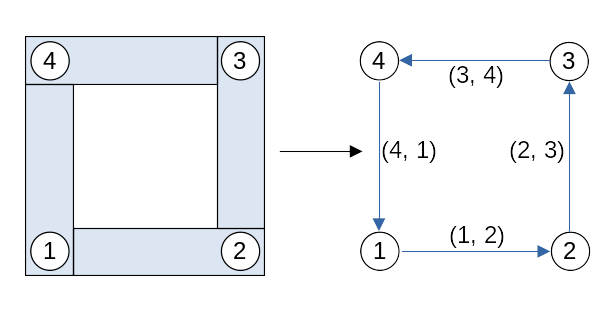
\includegraphics[width=\linewidth]{images/location_encoding.png}
    \caption{Standortenkodierung der Orte und Pfade.}
    \label{fig:location_encoding}
\end{figure}
\newline
Daraus wird die Komplexität und Genauigkeit dieser Ansätze deutlich.
Der Kantenansatz ist ein Kompromiss zwischen Genauigkeit und Komplexität.
Dabei bestimmt die Anzahl der zu klassifizierenden Standorte die Komplexität.
Zum einen ist gerade bei langen Pfaden eine geringe Auflösung im Vergleich zur Realposition des Objektes zu erwarten,
d. h. es ist unklar, ob sich das Objekt am Anfang, Ende oder in dazwischen befindet.
Zum anderen werden in einem zyklischen Graphen mindestens so viele Standorte, wie beim Knotenansatz verwendet.
Der Knotenansatz benötigt am wenigsten Standorte zur Enkodierung ist aber außerhalb der Standorte sehr ungenau.
Aus einer Historie von vorherigen Standorten kann aber ein möglicher Pfad inferiert werden,
allerdings können auch mehrere Pfade in Frage kommen, z. B. bei einer Gabelung.
Der kombinierte Ansatz enkodiert soviele Standorte wie beide Ansätze zusammen,
wodurch dieser Ansatz am komplexisten ist und am schlechtesten für große Routen skaliert.
Dafür ist die Auflösung des kombinierten Ansatzes so gut, wie eine diskrete Enkodierung es zulässt.
\newline
\newline
Ist in den aufgenommenen Trainingsdaten die Position des Objektes zum Zeitpunkt der Aufnahme der Sensorwerte bekannt,
so können die Standorte nach dem gewählten Enkodierungsansatz beliebig genau beschriftet werden.
Dies kann in einem Weiterverarbeitungsschritt nach der Aufnahme der Daten mit einer Karte von den Interessepunkten geschehen.
\newline
\newline
Bei der Evaluation in Kapitel \ref{sec:eval_anomalieerkennung} hat sich gezeigt, dass Anomalien besser erkannt werden können,
wenn die Auflösung des Enkodierungsansatzes hoch ist.